%!TEX root = ../thesis.tex
%*******************************************************************************
%*********************************** First Chapter *****************************
%*******************************************************************************

\chapter{Overview Of nano-scale heat transfer}  %Title of the First Chapter

\graphicspath{{Chapter1/}}

%********************************** %First Section  **************************************

%%%%%%%%%%%%%%%%%%%%%%%%%%%%%%%%%%%%%%%%%%%%%%%
%A roadmap
% 1. The studying condition of nano-scale heat transfer and the future development
% 2. Focus:The world of Compound Semiconductors
% 3. Result;The dream of tuning the heat
%%%%%%%%%%%%%%%%%%%%%%%%%%%%%%%%%%%%%%%%%%%%%%%%

\setlength{\epigraphwidth}{0.6\textwidth}
\epigraph{“Any sufficiently advanced technology is indistinguishable from magic.”}
{\textit{Arthur C. Clarke(British science fiction writer)}}

\section{Introduction}
The relentless decrease in the size of devices and structures, the increase in the operating speeds and frequencies, and the ever more aggressive thermal conditions imposed upon them requres sophisticated understanding and control of the thermal transport at the nano scale\cite{cahill2014nanoscale}.
While thermal performance itself is a key metric for several applications such as nuclear fuels, thermal barrier coatings, there are many other technologies for which the ability to manipulate heat is vital even though the primary goal of the structure is non-thermal. For example, progress in the control of thermal transport at the nanoscale is critical to continued advances in the density of information that can be stored in phase change memory devices and new
generations of magnetic storage that will use highly localized heat sources to reduce the coercivity
of magnetic media.\\
\indent Now, we will first give an exact definition of the term nanoscale and then give an introduction to the nanoscale heat conduction and especially heat conduction in interface. The term nanoscale is
interpreted liberally, embracing characteristic dimensions
ranging from the atomic up to sub-micron. Another way of
envisaging the definition of nanoscale is the regime in which
sub-continuum effects are important; that is, the system cannot
be adequately described by bulk transport properties and
continuum heat transport equations that do not explicitly
consider interfaces.
\section{Physical Mechanisms of nanoscale heat condcution}
Heat conduction in nanostructures is not the same as in macroscopic systems, where
it is characterised by Fourier’s law. In the latter case, the heat carriers can be visualised
as behaving like little beads with Brownian-like trajectories, i.e., suffering frequent and random changes of direction. These movements are due to collisions
between the carriers owing to their high density.
\subsection{Rarefaction,Surface Reflection and Transmission at Interfaces}
However, when this density decreases, the distance travelled by a heat particle between
two collisions can exceed the characteristic length scale of the structure. The
particle will then enter into more collisions with the walls of the system than with
its counterparts within the system. This regime is no longer Brownian, but ballistic,
because the particle will basically move in a straight line at constant speed between
consecutive reflections from the system walls Fig(\ref{fig:mingo}).\\
\begin{figure}[htbp!] 
\centering    
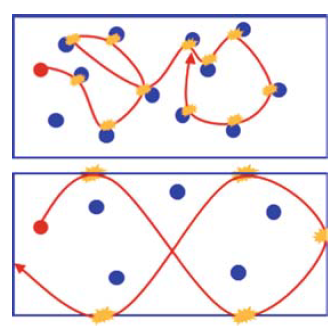
\includegraphics[width=0.4\textwidth]{1.png}
\caption[ballistic]{Path of a heat carrying particle (\textit{red} blob) in the diffusive regime (\textit{top}), where the carrier
density is high, and in the ballistic regime (\textit{bottom}), where the carrier density is low. The prevailing
mechanism in the diffusive case is interparticle interaction. In the ballistic case, it is particle–
surface interactions that dominate\cite{mingolbook}}
\label{fig:mingo}
\end{figure}{}

In a first approximation, reflection and transmission are assumed to be a linear
combination of the two extremes, specular and diffuse. The fraction of the incident
energy that is reflected specularly defines a coefficient called the specularity. But
while the particle on its straight line path is indeed treated as a particle, it is its
wavelike behaviour that governs its reflection or transmission. The specularity coefficient
will thus depend on the wavelength and polarisation of the particle, the
roughness of the surface, and the angle of incidence. It is therefore impossible to
account exhaustively for the full complexity of the physical mechanisms that contribute
to this coefficient, and it is generally treated as a floating parameter when
computations are carried out.\\
\indent This first rarefaction effect is often computed using the Boltzmann equation, which is exactly what we conduct with MC methods in Chapter 2.
\subsection{Confinement}
The word ‘particle’ is used to cover the more detailed reality of a localised wave
packet. This wave packet is made up of several waves in different resonant or normal
modes. It is the mode, the manner of vibration, that contains the energy of the
system. It is assumed to be a travelling wave, since the system is a bulk system and
much bigger than the lattice constant, i.e., the interatomic distance. The amplitudes
$u_n$ of these waves can be modelled by plane monochromatic waves, that is, complex
exponentials whose arguments contain the wave vectors $k$ and a time dependence associated with the frequency $\omega$:
\begin{equation*}
u_n=ue^{i(kx-\omega t)}
\end{equation*}
When modelling such modes, the boundary conditions are called Born–Von Karman
conditions: the wave arriving at one end will come back in by the other. It thus
propagates indefinitely in the same direction as long as it does not interact, and it
moves at a speed imposed by the speed of the given mode.\\
\indent Imagine now that the wave amplitude is annihilated at one end. This is what happens,
for example, at the bridge of a guitar or when an acoustic wave in a crystal
arrives at a free surface. The wave incident at this stopping point will be reflected
with reversal of its phase. The incident and reflected waves
can still be modelled by monochromatic plane waves, that is, complex exponentials
whose arguments contain wave vectors k with opposite signs, since the waves propagate
in opposite directions. Their superposition is thus modelled as a sum of two
exponentials, equal to the product of a cosine function whose argument depends on
the wave vector and a complex exponential defining the temporal phase:
\begin{equation*}
u_n ~ e^{i(kx-\omega t)}+e^{i(-kx-\omega t)}= cos(kx)e^{-i \omega t}
\end{equation*}
The zeros of the cosine function do not depend on time and define the nodes of a
stationary wave. The vanishing of the amplitude at the boundary $x=L$ requires $kL=\pi /2+n2\pi$, where $n$ is an integer\cite{mingo2005carbon}. The wavelengths are thus $L/(n+1/4)$, defining
the normal modes of the cavity formed by the structure. If the width $L$ varies, then
the wavelengths will also vary. New eigenmodes specific to the nanostructure thus
form.\\
\indent This transformation of the travelling normalmodes into stationary normalmodes
is the second non-Fourier effect, referred to as confinement. By definition, these
stationary waves have zero propagation speed. As the heat flux is proportional to
the speed, the contribution of such stationary modes to heat transfer also vanishes The dispersion curves giving the frequency as a function of the wave vector are
therefore flat, because their slope is given by the mode speed, as shown in Fig(\ref{fig:mingopic}).
\begin{figure}[htbp!] 
\centering    
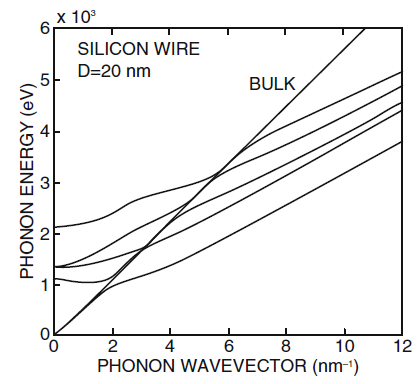
\includegraphics[width=0.4\textwidth]{2.png}
\caption[confinement]{Dispersion curves for the phonons in a silicon nanowire of diameter 20 nm (\textit{continuous
lines}). Small slopes and low group velocities correspond to small phonon wave vectors or long
wavelengths as a result of confinement. Each branch is related to the projection of an oblique mode
onto the wire axis. The bulk dispersion curve is shown by the \textit{dashed line}.\cite{mingolbook}}
\label{fig:mingopic}
\end{figure}{}
\subsection{Density of States and Dimensionality}
As can be shown from Fig(\ref{fig:mingopic}), confinement modifies the distribution of the modes
as a function of frequency. The number of modes in a given frequency interval$[\omega, \omega + d \omega]$ or wave vector interval $[\textbf{k},\textbf{k}+d^3 \textbf{k}]$ is called the density of states $D(\omega)$ or $D(k)$, respectively.\\
\indent The directions of the vibrations in a crystal cover the whole space, and so do the
directions of the wave vectors. The density of states in the bulk is thus proportional
to a volume element, let us say an element in the form of a spherical shell, i.e., $D(k) \propto k^2 dk$. If now the vibrations only build up in two dimensions, as in a graphene
film, the density of states is proportional to a surface element, i.e., $D(k) \propto k^2 dk$.Finally, in the case of a nanowire, where the vibrations can only propagate in one
direction, the density of states is proportional to a length element, i.e., $D(k) \propto k dk$.\\
\indent Since the thermal conductivity is proportional to the heat capacity, and
hence to the density of states, the dimensionality of the structure has a significant
impact on heat transfer. 

%\section{Interface}
%After discussing all the three non-Fourier effects and getting a overall view of the nanoscale heat transfer, we will turn to focusing on the topic of interface, which becomes increasingly important on small length scales.  

\section{Solid-State Lighting: Focusing III-V semiconductors}

The interactive progress in semiconductor science and technology has transformed and continues to transform both our scientific understanding of the universe and the technologies with which we live our daily lives\cite{LEDblue}. A testament to this are the seven Physics Nobel Prizes listed in Fig(\ref{fig:LEDnobel}) that have been awarded in the broad area of semiconductors.
\begin{figure}[htbp!] 
\centering    
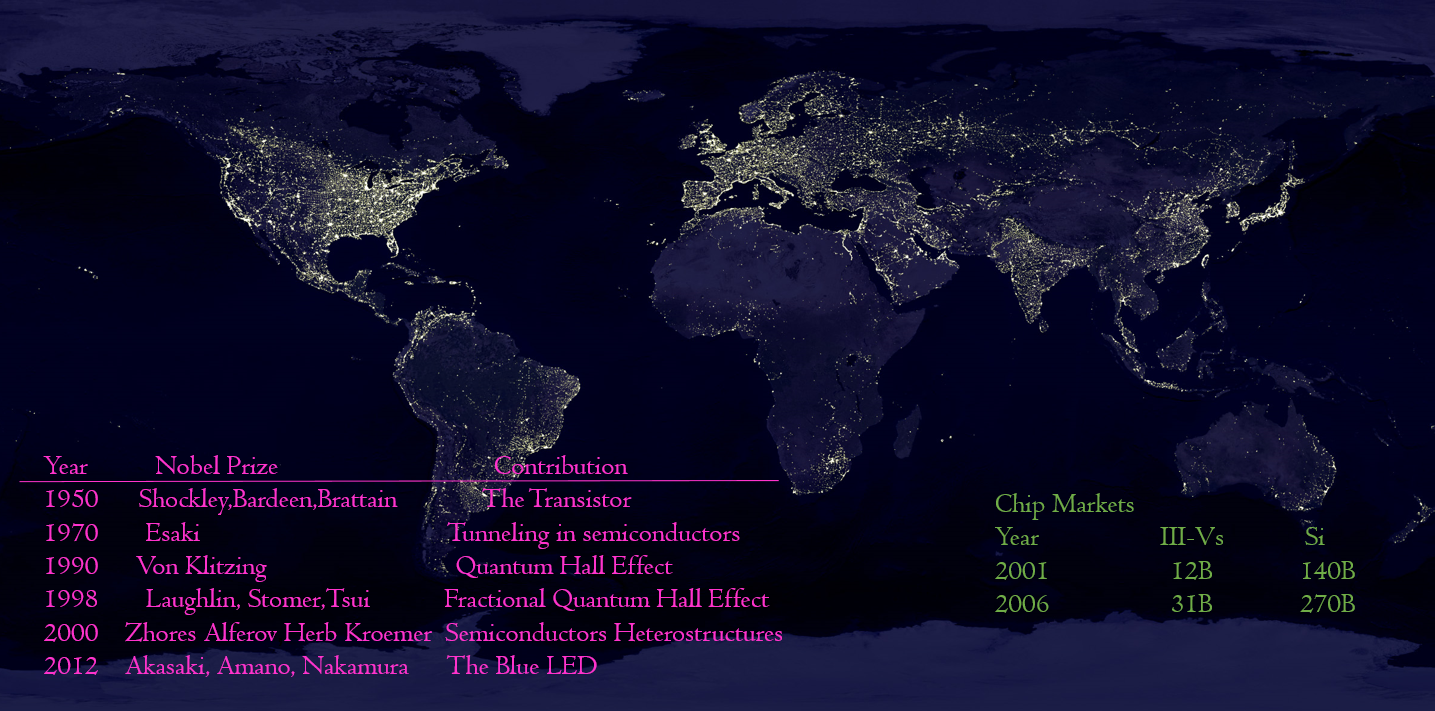
\includegraphics[width=0.8\textwidth]{NASA.png}
\caption[semiconductorsNobel]{Timeline of Physics Nobel Prizes in semiconductor science and technology}
\label{fig:LEDnobel}
\end{figure}{}
Some of the Prizes were for technology
breakthroughs – as with research
surrounding Si planar processing
and the integrated circuit.
Some of the Prizes were for science
breakthroughs – as with research
surrounding the integer and
fractional quantum Hall effects. And
some were for nearly simultaneous
science and technology breakthroughs
– as with the transistor.\\
\indent The most recent 2014 Physics Nobel Prize, for the blue light-emiting diode(LED), is clearly for a technology breakthrough. Indeed, this makes it possible to gain relaible and clean light and thus bring about a Solid-State Lighting revolution.Because artificial lighting is so critical to humanity and consumes so
much energy (approximately 6.5\% of
the world’s primary energy and 16\%
of the world’s total generated electrical
energy \cite{LEDworld}), the energy savings
potential of SSL is huge.\\
\indent During all the types of semi-conductors, when we talk about Optoelectronics, the III-Vs can be very unique.
The uniqueness and practical importance of the
compound III-V semiconductors stems from their
balancing of these competing trends. They are
polar enough to be direct-bandgap semiconductors,
with the accompanying strong interactions with
photons useful for optoelectronics and the low
electron masses useful for high-speed electronics.
But they are not so polar that they cannot be p-type
doped or that they suffer from too-high defect
densities.Thus, III-Vs semi-conductors gain vital importance in the area of LED or other Optoelectronics.\\
\indent Also, as we have mentioned in the Intro, the rapid development of Optoelectronics especially the nano III-V structures demands a deep understanding of the phonon transport and then tuning the heat condcution, which is the basic background of our whole research. So in this part, we will then focus on the most important part of the nano structures-interface and will continue this topic in late chapters.
% \section{Thermal Conductance of Inteface}
% %\subsubsection{Vibrational thermal energy transport at interfaces}
% Interfaces play a key role in the thermal behavior of nanostructures. At small scales, interfaces have the potential to become the dominant resistance to heat conduction, which impedes the progress towards achieving improved performance in nano-electronics\cite{pop2010energy}, nano-optoelectronics\cite{tien1994challenges}, or energy conversion devices such as multi-junction solar cells\cite{min2009thermal,katz2006effects}.
% A thermal boundary resistance is found for the heat flow
% between two materials in contact along a planar interface.
% The heat flow is perpendicular to the planar interface
% \begin{equation}
% J_Q=G \Delta T
% \end{equation}
% where $\Delta T$ is the small temperature difference between the two sides of the interface, and $G$ is the boundary conductance; $G$ has the units of power per aera per degree.\\
% A common interface in thermal transport is bettween two insulators. Then, the heat is carried only by phonons. The accoustic model(AMM)\cite{little1959transport} and diffusive mismatch model(DMM)\cite{swartz1989thermal} have traditionally provided a basis for understanding interfacial thermal resistance. These models provide prescriptions for calculating the transmission coefficient of a phonon with which the interfacial conductance can be obtained by appropriate summations over all phonons\cite{young1989lattice,swartz1989thermal}.\\
% As a continuum model, the AMM assumes that phonons
% undergo specular reflection or transmission at the interface.
% This model is valid in the long-wavelength limit, where
% due to their small details compared to the incident phonon
% wavelength, interfaces are seen as sharp. The DMM, on
% the other hand, assumes not only purely diffuse scattering
% at the interface, but also an equivalence between phonon
% reflectance from one side to the transmittance from the other.
% This model, as opposed to AMM, is valid for very rough or
% dirty interfaces and short-wavelength phonons. Neither AMM
% nor DMM consistently predict interface thermal boundary
% resistance.\\
% For the late discussion it should be pointed out here that while both AMM and DMM provide values
% for transmission coefficients, they calculate them purely
% based on the bulk properties of the two solids forming the
% interface; thus they do not account explicitly for the strength of the interfacial bonding. 

\section{My Oric Study}
After giving the introduction above, we can conclude that nanoscale thermal transport plays an important role in the functionality and the reliability of nano-enabled systems. However, we must realize that the understanding of nanoscale thermal transpoat is still in its infancy.\\
\indent The key to the difference in thermal transport at nanoscale from that at macroscale is the scattering of energy carriers at interfaces. And we have also introduced the two well-known model DMM and AMM which have been widely-used to describe the phonon properties in interfaces, however, in many realistic systems, just the macroscopic properties, which the two models only contain, such as interfacial thermal resistance and the reduced thermal conductvity of nanostructures, could not caputure all the underlying physics\cite{yang2004thermal,yang2005thermal}.For example, a large-scale nano-bulk system with multiple interfaces such as intergrated circuits(\textbf{ICs})\cite{IC} and nanocomposites\cite{yang2005thermal} will call for a better set of variables and simulation tools to describe such a system. Empirical approaches are the Boltzmann transport equation-based determinstic andstochastic approches, which could potentially link the length scales from a few nanometers to the macroscale\cite{LD2}. And we will also conduct a MC simulation based on phonon BTE mainly to recover the picture of the nano-scale heat conduction and in this work we also consider the effect of the internal heat source which can be a good model for many actual nano-thermal devices, for example, chips.\\
\indent Although such simulations gain great success in several topics, tools like MC simulation require input parameters that must be obtained at even smaller length scales, such as the phonon relaxation time, phonon dispersion, and phonon transmission coefficent at interfaces(These can be seen from Chapter 2 and Appendix A ). Most of these input parameters(material properties at atmistic scale) are energy or wavevector(actually these two are same). More importantly, various factors, such as material differences, atomic reconstruction at the interfacial region, dislocations, defects, strain fields, and the size of the structures, could affect these parameters, including phonon transmission across interfaces of dissimilar materials\cite{li2012size}.\\
\indent Modeling of phonon transmission across material interfaces has been challenging. The acoustic mismatch model(AMM) and diffuse mismatch model(DMM) are often used for the calculation of phonon transmission as input parameters for Boltzmann equation solvers\cite{DMM}.
The AMM considers long-wavelength phonons and uses the acoustic impedances of the two adjacent materials for the calculation of phonon transmission. The model is strictly valid only at low temperatures. Phonon scattering at interfaces is assumed to be completely diffusive in the DMM\cite{DMM},which relates the
phonon transmission to the mismatch of the phonon density
of states (DOS) of two materials. The DMM better predicts
phonon transmission at high temperature or across rough
interfaces. Although the AMM and DMM have been used
exclusively for BTE solutions and for explaining experimental
data, neither the AMM nor the DMM can accurately capture
the underlying physics of phonon dynamics and transport
across material interfaces.\\
\indent Significant progress has been made recently in studying	phonon transmission based on atomistic simulations. The
phonon wavepacket method\cite{schelling2002phonon} was developed to study
phonon transmission based on molecular dynamics (MD)
simulations. In this method, a phonon wavepacket is
initiated in one material and propagates across the interface.
Wavefunctions with specified wavevector and frequency are
used to assign the initial displacement and velocity of the
atoms. The transmission coefficient is calculated by the
ratio of the total energies (both potential and kinetic) of
the atoms on the two sides of an interface.However, usually the
simulation domain is very large in the direction perpendicular
to the interface\cite{schelling2002phonon,sun2010molecular}.For example, a size of 543 nm
is used in work\cite{schelling2002phonon}, and only one phonon transmission data
point corresponding to a specific phonon wavevector can be
obtained in one run of MD simulation.It is rather costly for obtaining the phonon transmission for all phonon modes.\\
\indent Linear lattice dynamics\cite{stoner1992measurements,zhao2005lattice} was proposed to
calculate phonon transmission using the lattice dynamical
equation derived for the atoms at the interface. Under the
harmonic approximation, the frequency of the transmitted
and reflected phonons does not change. With this boundary
condition, the wavefunctions of the reflected and transmitted
phonons can be solved and then the phonon transmission
is calculated based on the energies of the reflected and
transmitted phonon waves across the interface.\\
\indent Instead of solving for phonon waves in the linear
lattice dynamics method, the atomistic Green’s function
(AGF) approach solves for the response of the system
under small perturbations. In the AGF approach, a lattice
system is divided into decoupled sub-systems. The Green’s
functions of the decoupled sub-systems are obtained first
and the Green’s function of the coupled system is then
calculated by linking the Green’s functions of the decoupled
sub-systems. In this way, if there is any change in one of
the decoupled sub-systems, only the Green’s function of
this decoupled sub-system needs to be recalculated and the
new Green’s function of the whole system can be relatively
easily calculated by replacing the Green’s function of this
sub-system, which is more computationally efficient than
the linear lattice dynamics method. A number of interfacial
structures have been studied using the AGF approach,
including low-dimensional molecular chains, coated silicon
nanowires (NWs), amide-linked carbon nanotubes, latticematched
Si/Ge interfaces and rough interfaces of two
face-centered cubic (fcc) lattices\cite{ozpineci2001quantum,zhao2009phonon,dhar2006heat}.\\
\indent As we have mentioned above, it is far from enough to only consider bulk or macroscale properties to explain the interface mechanism, however, few studies have addressed this problem. So in our work, whose background is Optoelectronics, we set the final goal to further understand the deeper mechanism and physics in interface and this report focus on the phonon properties in III-V semi-conductors and also the heat transfer in these nano-structures. The paper is organized as follows.
In Chapter 2, the phonon MC method with the internal heat source is presented to mainly show the different temperature profile and the nano-heattransfer effects. In Chapter 3, we present the phonon transmission across the III-V semi-conductors interfaces. In Chapter 4, concludes the work and list the two undergoing work on that issue in our further study.

